
%% bare_conf.tex
%% V1.3
%% 2007/01/11
%% by Michael Shell
%% See:
%% http://www.michaelshell.org/
%% for current contact information.
%%
%% This is a skeleton file demonstrating the use of IEEEtran.cls
%% (requires IEEEtran.cls version 1.7 or later) with an IEEE conference paper.
%%
%% Support sites:
%% http://www.michaelshell.org/tex/ieeetran/
%% http://www.ctan.org/tex-archive/macros/latex/contrib/IEEEtran/
%% and
%% http://www.ieee.org/

%%*************************************************************************
%% Legal Notice:
%% This code is offered as-is without any warranty either expressed or
%% implied; without even the implied warranty of MERCHANTABILITY or
%% FITNESS FOR A PARTICULAR PURPOSE! 
%% User assumes all risk.
%% In no event shall IEEE or any contributor to this code be liable for
%% any damages or losses, including, but not limited to, incidental,
%% consequential, or any other damages, resulting from the use or misuse
%% of any information contained here.
%%
%% All comments are the opinions of their respective authors and are not
%% necessarily endorsed by the IEEE.
%%
%% This work is distributed under the LaTeX Project Public License (LPPL)
%% ( http://www.latex-project.org/ ) version 1.3, and may be freely used,
%% distributed and modified. A copy of the LPPL, version 1.3, is included
%% in the base LaTeX documentation of all distributions of LaTeX released
%% 2003/12/01 or later.
%% Retain all contribution notices and credits.
%% ** Modified files should be clearly indicated as such, including  **
%% ** renaming them and changing author support contact information. **
%%
%% File list of work: IEEEtran.cls, IEEEtran_HOWTO.pdf, bare_adv.tex,
%%                    bare_conf.tex, bare_jrnl.tex, bare_jrnl_compsoc.tex
%%*************************************************************************

% *** Authors should verify (and, if needed, correct) their LaTeX system  ***
% *** with the testflow diagnostic prior to trusting their LaTeX platform ***
% *** with production work. IEEE's font choices can trigger bugs that do  ***
% *** not appear when using other class files.                            ***
% The testflow support page is at:
% http://www.michaelshell.org/tex/testflow/



% Note that the a4paper option is mainly intended so that authors in
% countries using A4 can easily print to A4 and see how their papers will
% look in print - the typesetting of the document will not typically be
% affected with changes in paper size (but the bottom and side margins will).
% Use the testflow package mentioned above to verify correct handling of
% both paper sizes by the user's LaTeX system.
%
% Also note that the "draftcls" or "draftclsnofoot", not "draft", option
% should be used if it is desired that the figures are to be displayed in
% draft mode.
%
\documentclass[conference,12pt]{IEEEtran}
% Add the compsoc option for Computer Society conferences.
%
% If IEEEtran.cls has not been installed into the LaTeX system files,
% manually specify the path to it like:
% \documentclass[conference]{../sty/IEEEtran}





% Some very useful LaTeX packages include:
% (uncomment the ones you want to load)


% *** MISC UTILITY PACKAGES ***
%
%\usepackage{ifpdf}
% Heiko Oberdiek's ifpdf.sty is very useful if you need conditional
% compilation based on whether the output is pdf or dvi.
% usage:
% \ifpdf
%   % pdf code
% \else
%   % dvi code
% \fi
% The latest version of ifpdf.sty can be obtained from:
% http://www.ctan.org/tex-archive/macros/latex/contrib/oberdiek/
% Also, note that IEEEtran.cls V1.7 and later provides a builtin
% \ifCLASSINFOpdf conditional that works the same way.
% When switching from latex to pdflatex and vice-versa, the compiler may
% have to be run twice to clear warning/error messages.






% *** CITATION PACKAGES ***
%
%\usepackage{cite}
% cite.sty was written by Donald Arseneau
% V1.6 and later of IEEEtran pre-defines the format of the cite.sty package
% \cite{} output to follow that of IEEE. Loading the cite package will
% result in citation numbers being automatically sorted and properly
% "compressed/ranged". e.g., [1], [9], [2], [7], [5], [6] without using
% cite.sty will become [1], [2], [5]--[7], [9] using cite.sty. cite.sty's
% \cite will automatically add leading space, if needed. Use cite.sty's
% noadjust option (cite.sty V3.8 and later) if you want to turn this off.
% cite.sty is already installed on most LaTeX systems. Be sure and use
% version 4.0 (2003-05-27) and later if using hyperref.sty. cite.sty does
% not currently provide for hyperlinked citations.
% The latest version can be obtained at:
% http://www.ctan.org/tex-archive/macros/latex/contrib/cite/
% The documentation is contained in the cite.sty file itself.






% *** GRAPHICS RELATED PACKAGES ***
%
\ifCLASSINFOpdf
  \usepackage[pdftex]{graphicx}
  % declare the path(s) where your graphic files are
  \graphicspath{{./images/}}
  % and their extensions so you won't have to specify these with
  % every instance of \includegraphics
  % \DeclareGraphicsExtensions{.pdf,.jpeg,.png}
\else
  % or other class option (dvipsone, dvipdf, if not using dvips). graphicx
  % will default to the driver specified in the system graphics.cfg if no
  % driver is specified.
  % \usepackage[dvips]{graphicx}
  % declare the path(s) where your graphic files are
  % \graphicspath{{../eps/}}
  % and their extensions so you won't have to specify these with
  % every instance of \includegraphics
  % \DeclareGraphicsExtensions{.eps}
\fi
% graphicx was written by David Carlisle and Sebastian Rahtz. It is
% required if you want graphics, photos, etc. graphicx.sty is already
% installed on most LaTeX systems. The latest version and documentation can
% be obtained at: 
% http://www.ctan.org/tex-archive/macros/latex/required/graphics/
% Another good source of documentation is "Using Imported Graphics in
% LaTeX2e" by Keith Reckdahl which can be found as epslatex.ps or
% epslatex.pdf at: http://www.ctan.org/tex-archive/info/
%
% latex, and pdflatex in dvi mode, support graphics in encapsulated
% postscript (.eps) format. pdflatex in pdf mode supports graphics
% in .pdf, .jpeg, .png and .mps (metapost) formats. Users should ensure
% that all non-photo figures use a vector format (.eps, .pdf, .mps) and
% not a bitmapped formats (.jpeg, .png). IEEE frowns on bitmapped formats
% which can result in "jaggedy"/blurry rendering of lines and letters as
% well as large increases in file sizes.
%
% You can find documentation about the pdfTeX application at:
% http://www.tug.org/applications/pdftex





% *** MATH PACKAGES ***
%
\usepackage[cmex10]{amsmath}
% A popular package from the American Mathematical Society that provides
% many useful and powerful commands for dealing with mathematics. If using
% it, be sure to load this package with the cmex10 option to ensure that
% only type 1 fonts will utilized at all point sizes. Without this option,
% it is possible that some math symbols, particularly those within
% footnotes, will be rendered in bitmap form which will result in a
% document that can not be IEEE Xplore compliant!
%
% Also, note that the amsmath package sets \interdisplaylinepenalty to 10000
% thus preventing page breaks from occurring within multiline equations. Use:
%\interdisplaylinepenalty=2500
% after loading amsmath to restore such page breaks as IEEEtran.cls normally
% does. amsmath.sty is already installed on most LaTeX systems. The latest
% version and documentation can be obtained at:
% http://www.ctan.org/tex-archive/macros/latex/required/amslatex/math/





% *** SPECIALIZED LIST PACKAGES ***
%
%\usepackage{algorithmic}
% algorithmic.sty was written by Peter Williams and Rogerio Brito.
% This package provides an algorithmic environment fo describing algorithms.
% You can use the algorithmic environment in-text or within a figure
% environment to provide for a floating algorithm. Do NOT use the algorithm
% floating environment provided by algorithm.sty (by the same authors) or
% algorithm2e.sty (by Christophe Fiorio) as IEEE does not use dedicated
% algorithm float types and packages that provide these will not provide
% correct IEEE style captions. The latest version and documentation of
% algorithmic.sty can be obtained at:
% http://www.ctan.org/tex-archive/macros/latex/contrib/algorithms/
% There is also a support site at:
% http://algorithms.berlios.de/index.html
% Also of interest may be the (relatively newer and more customizable)
% algorithmicx.sty package by Szasz Janos:
% http://www.ctan.org/tex-archive/macros/latex/contrib/algorithmicx/




% *** ALIGNMENT PACKAGES ***
%
%\usepackage{array}
% Frank Mittelbach's and David Carlisle's array.sty patches and improves
% the standard LaTeX2e array and tabular environments to provide better
% appearance and additional user controls. As the default LaTeX2e table
% generation code is lacking to the point of almost being broken with
% respect to the quality of the end results, all users are strongly
% advised to use an enhanced (at the very least that provided by array.sty)
% set of table tools. array.sty is already installed on most systems. The
% latest version and documentation can be obtained at:
% http://www.ctan.org/tex-archive/macros/latex/required/tools/


%\usepackage{mdwmath}
%\usepackage{mdwtab}
% Also highly recommended is Mark Wooding's extremely powerful MDW tools,
% especially mdwmath.sty and mdwtab.sty which are used to format equations
% and tables, respectively. The MDWtools set is already installed on most
% LaTeX systems. The lastest version and documentation is available at:
% http://www.ctan.org/tex-archive/macros/latex/contrib/mdwtools/


% IEEEtran contains the IEEEeqnarray family of commands that can be used to
% generate multiline equations as well as matrices, tables, etc., of high
% quality.


%\usepackage{eqparbox}
% Also of notable interest is Scott Pakin's eqparbox package for creating
% (automatically sized) equal width boxes - aka "natural width parboxes".
% Available at:
% http://www.ctan.org/tex-archive/macros/latex/contrib/eqparbox/





% *** SUBFIGURE PACKAGES ***
\usepackage[tight,footnotesize]{subfigure}
\usepackage{wrapfig} 
% subfigure.sty was written by Steven Douglas Cochran. This package makes it
% easy to put subfigures in your figures. e.g., "Figure 1a and 1b". For IEEE
% work, it is a good idea to load it with the tight package option to reduce
% the amount of white space around the subfigures. subfigure.sty is already
% installed on most LaTeX systems. The latest version and documentation can
% be obtained at:
% http://www.ctan.org/tex-archive/obsolete/macros/latex/contrib/subfigure/
% subfigure.sty has been superceeded by subfig.sty.



%\usepackage[caption=false]{caption}
%\usepackage[font=footnotesize]{subfig}
% subfig.sty, also written by Steven Douglas Cochran, is the modern
% replacement for subfigure.sty. However, subfig.sty requires and
% automatically loads Axel Sommerfeldt's caption.sty which will override
% IEEEtran.cls handling of captions and this will result in nonIEEE style
% figure/table captions. To prevent this problem, be sure and preload
% caption.sty with its "caption=false" package option. This is will preserve
% IEEEtran.cls handing of captions. Version 1.3 (2005/06/28) and later 
% (recommended due to many improvements over 1.2) of subfig.sty supports
% the caption=false option directly:
%\usepackage[caption=false,font=footnotesize]{subfig}
%
% The latest version and documentation can be obtained at:
% http://www.ctan.org/tex-archive/macros/latex/contrib/subfig/
% The latest version and documentation of caption.sty can be obtained at:
% http://www.ctan.org/tex-archive/macros/latex/contrib/caption/




% *** FLOAT PACKAGES ***
%
%\usepackage{fixltx2e}
% fixltx2e, the successor to the earlier fix2col.sty, was written by
% Frank Mittelbach and David Carlisle. This package corrects a few problems
% in the LaTeX2e kernel, the most notable of which is that in current
% LaTeX2e releases, the ordering of single and double column floats is not
% guaranteed to be preserved. Thus, an unpatched LaTeX2e can allow a
% single column figure to be placed prior to an earlier double column
% figure. The latest version and documentation can be found at:
% http://www.ctan.org/tex-archive/macros/latex/base/



%\usepackage{stfloats}
% stfloats.sty was written by Sigitas Tolusis. This package gives LaTeX2e
% the ability to do double column floats at the bottom of the page as well
% as the top. (e.g., "\begin{figure*}[!b]" is not normally possible in
% LaTeX2e). It also provides a command:
%\fnbelowfloat
% to enable the placement of footnotes below bottom floats (the standard
% LaTeX2e kernel puts them above bottom floats). This is an invasive package
% which rewrites many portions of the LaTeX2e float routines. It may not work
% with other packages that modify the LaTeX2e float routines. The latest
% version and documentation can be obtained at:
% http://www.ctan.org/tex-archive/macros/latex/contrib/sttools/
% Documentation is contained in the stfloats.sty comments as well as in the
% presfull.pdf file. Do not use the stfloats baselinefloat ability as IEEE
% does not allow \baselineskip to stretch. Authors submitting work to the
% IEEE should note that IEEE rarely uses double column equations and
% that authors should try to avoid such use. Do not be tempted to use the
% cuted.sty or midfloat.sty packages (also by Sigitas Tolusis) as IEEE does
% not format its papers in such ways.





% *** PDF, URL AND HYPERLINK PACKAGES ***
%
%\usepackage{url}
% url.sty was written by Donald Arseneau. It provides better support for
% handling and breaking URLs. url.sty is already installed on most LaTeX
% systems. The latest version can be obtained at:
% http://www.ctan.org/tex-archive/macros/latex/contrib/misc/
% Read the url.sty source comments for usage information. Basically,
% \url{my_url_here}.





% *** Do not adjust lengths that control margins, column widths, etc. ***
% *** Do not use packages that alter fonts (such as pslatex).         ***
% There should be no need to do such things with IEEEtran.cls V1.6 and later.
% (Unless specifically asked to do so by the journal or conference you plan
% to submit to, of course. )


% correct bad hyphenation here
\hyphenation{op-tical net-works semi-conduc-tor}
\usepackage{listings}
\usepackage{algorithmic}
\usepackage[boxed]{algorithm}


\begin{document}
%
% paper title
% can use linebreaks \\ within to get better formatting as desired
\title{\vspace{-0.05\textheight}System Design Project Final Report}


% author names and affiliations
% use a multiple column layout for up to three different
% affiliations
\author{\vspace{-0.05\textheight}\IEEEauthorblockN{Seyed Behzad Tabibian, Calum Jackson}
\IEEEauthorblockA{Group12 - School of Informatics}}

% conference papers do not typically use \thanks and this command
% is locked out in conference mode. If really needed, such as for
% the acknowledgment of grants, issue a \IEEEoverridecommandlockouts
% after \documentclass

% for over three affiliations, or if they all won't fit within the width
% of the page, use this alternative format:
% 
%\author{\IEEEauthorblockN{Michael Shell\IEEEauthorrefmark{1},
%Homer Simpson\IEEEauthorrefmark{2},
%James Kirk\IEEEauthorrefmark{3}, 
%Montgomery Scott\IEEEauthorrefmark{3} and
%Eldon Tyrell\IEEEauthorrefmark{4}}
%\IEEEauthorblockA{\IEEEauthorrefmark{1}School of Electrical and Computer Engineering\\
%Georgia Institute of Technology,
%Atlanta, Georgia 30332--0250\\ Email: see http://www.michaelshell.org/contact.html}
%\IEEEauthorblockA{\IEEEauthorrefmark{2}Twentieth Century Fox, Springfield, USA\\
%Email: homer@thesimpsons.com}
%\IEEEauthorblockA{\IEEEauthorrefmark{3}Starfleet Academy, San Francisco, California 96678-2391\\
%Telephone: (800) 555--1212, Fax: (888) 555--1212}
%\IEEEauthorblockA{\IEEEauthorrefmark{4}Tyrell Inc., 123 Replicant Street, Los Angeles, California 90210--4321}}




% use for special paper notices
%\IEEEspecialpapernotice{(Invited Paper)}




% make the title area
\maketitle


%\begin{abstract}
%\boldmath
%The abstract goes here.
%\end{abstract}
% IEEEtran.cls defaults to using nonbold math in the Abstract.
% This preserves the distinction between vectors and scalars. However,
% if the conference you are submitting to favors bold math in the abstract,
% then you can use LaTeX's standard command \boldmath at the very start
% of the abstract to achieve this. Many IEEE journals/conferences frown on
% math in the abstract anyway.

% no keywords




% For peer review papers, you can put extra information on the cover
% page as needed:
% \ifCLASSOPTIONpeerreview
% \begin{center} \bfseries EDICS Category: 3-BBND \end{center}
% \fi
%
% For peerreview papers, this IEEEtran command inserts a page break and
% creates the second title. It will be ignored for other modes.
\IEEEpeerreviewmaketitle
	

\newcommand{\revi}[1]{ \texttt{rev.#1} }
\vspace{-3 mm}
\section{Introduction}

This report will document the creation of our group’s robot for the System Design Project and evaluate the effectiveness and success of our methods. 
The aim of the project was to create a robot which could compete in a one-on-one football match against another robot. This report will explain how we organised our group, how we built the robot, the strategy we created to control the robot, how a vision system was implemented, and the implementation of a simulator.

Our aims for the project were to create a fast, lightweight robot alongside a effective planning algorithm to control it. Next to this, we also required:
\begin{itemize}
\item A vision system to convey the on-pitch data
\item A simulator for use in testing strategies
\end{itemize}

\vspace{-1 mm}
\section{Robot Construction}

Since our earliest robot designs, our design philosophy was to have a robust, lightweight and fast robot, which would be able to outmanoeuvre opponents on the pitch whilst being robust enough to withstand collisions with bigger opponents and walls. 

Reviewing the archives of previous SDP years, as well as closely following the developing designs of the other groups in our year, showed that this simple strategy was one that had been rejected, or possibly overlooked, by almost all other groups over time. Instead, designs that were favoured featured box-like structures with a lot of extra weight and a lack of agility. Due to the success of the previous years winners, holonomic wheels were considered, but were rejected due to not providing sufficient advantages to outweigh the extra effort necessary in their implementation, especially when this effort could be focused into other equally important areas such as strategy and vision, which we believed would be important in the final games. We also believed that a well designed wheel base, using non-holonomic differential drive wheels would allow for an equally manoeuvrable robot if used with an effective movement algorithm.

Researching into gears discovered a 3 - 10 ratio would make the robot up to three times faster than if the wheels were connected directly to the motors\footnote{http://www.ecst.csuchico.edu/\%7Ejuliano/csci224/Slides/03\%20-\%20Gears\%20Pulleys\%20Wheels\%20Tires.pdf}. Once gears were incorporated on the robot, whilst improving the speed as predicted,  they did affect the straight line ability of the robot, as shown below:
\begin{table}[ht]
\caption{Distance off-line (Running for 10seconds)}
\centering
\begin{tabular}{c c}
\hline\hline
Speed (rpm) & Off-Centre (mm) \\
1.5 & 82 \\
3 & 216 \\
4.5 & 850 \\
6 & N/A - Span in Circles \\
\hline\hline
\end{tabular}
\label{table:offline}
\end{table}
Clearly increased speeds led to massive offsets in travelling in a straight line. After testing multiple different options, including changing caster wheels, using ball-bearings, and putting the motors at the front, back and centre of the robot, it was eventually realised that the robot would diverge from its path whilst moving forwards, but would travel in a relatively straight line whilst reversing (at the same speed). Therefore a simple solution was to switch the direction which the motors faced (i.e. motors reversed $\rightarrow$ robot moved forward, and vice-versa). This led to much improved results:
\begin{table}[ht]
\caption{Distance off-line 2 (Running for 10seconds)}
\centering
\begin{tabular}{c c}
\hline\hline
Speed (rpm) & Off-Centre (mm) \\
1.5 & 0 \\
3 & 4 \\
4.5 & 10\\
6 & 46\\
\hline\hline
\end{tabular}
\label{table:online}
\end{table}

During the early stages of the build process we did not take into account that we were designing an actively controlled system, where robot’s path is being altered with every vision frame processed. Therefore these reduced discrepancies could be managed by the programming of the movement.
By the end of its development, despite its small, slight appearance, our robot was consistently one of the sturdier designs in the competition, only once losing a single piece from its structure due to a collision on the pitch.  Our fast, agile design also proved to be effective alongside our robust strategy, as we went on to achieve a semi-final position in all the friendly tournaments, before unfortunately being knocked out in the quarter finals on the final day. We were also among the teams with the highest number of total goals scored across all of our played matches, 16 in 8 matches!
\section{Strategy}

The main focus was to create an attacking strategy which would utilise the speed of the robot. The strategy was split into two sections, the high level areas (where the robot will move to, when to kick, dribble etc), and the lower level areas (coding the movement of the robot).

\subsection{High Level Strategy}
Initially we created a simple state system strategy, which checked the current on-pitch situation (using the data sent from the camera) and decided the appropriate strategy to run. The state system approach was used because new states could be added easily, allowing for multiple strategies.
Our strategy was based on defining a point to move towards. A point class was created, holding the x,y co-ordinates of points on the pitch. This class was extended to create instances of the robot, ball, goal, and any other necessary points for use in the strategy.


An optimum point was implemented (Algorithm 1), which would be a defined distance behind the ball at the same angle as the ball to goal angle, such that the robot would move to this point, and then to the ball, to ensure the robot was facing the goal when it reached the ball. This worked well in practice, working everytime when the robot was behind the ball, and 9/10 times when the robot was inbetween the goal and the ball (i.e. had to navigate around the ball).

\begin{algorithm}
\caption{Caclulate Optimum Point}
\label{optimumPoint}
\begin{algorithmic}[1]
\STATE $threshold \gets 70$
\STATE $(x_{1}, y_{1}) \gets ball (x, y)$
\STATE $(x_{2}, y_{2}) \gets goal (x, y)$
\STATE $ballGoalAngle = atan2( (y_{2} - y_{1}), (x_{2} - x_{1}) )$
%\STATE $hyp = \sqrt{\alpha^{2} + threshold^{2}}$
%\STATE $\theta = \sin(\frac{100}{hyp})$
\STATE $xOffset = threshold(\cos(ballGoallAngle)$
\STATE $yOffset = threshold(\sin(ballGoalAngle))$
\STATE $(x_{3}, y_{3}) = (x_{1} - xOffset, y_{1} - yOffset)$
\RETURN $(x_{3}, y_{3})$
\end{algorithmic}
\end{algorithm}

This function was later abstracted to a higher level, modifying the function to take any two points and return the angle between them, to increase its range and decrease repetition of similar code. \linebreak

The next target was to be able to navigate around objects. Points were used again, utilised in a function which would calculate an avoidance point at a $90^{\circ}$ angle and a defined distance from the object to avoid. The function would return the avoidance point, and the robot would move to it. \\
This function was dynamic, and the point would move as the robot moved, allowing the robot to navigate the object more smoothly.\\
The function calculated the avoid point using trigonometry, as shown in Algorithm 2 and the following diagram:
\begin{center}
\begin{figure}[htp]
\leavevmode
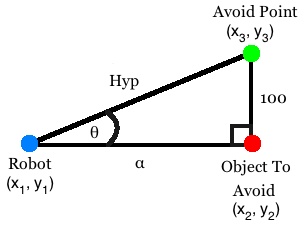
\includegraphics[scale=0.6]{images/AvoidPoints.png}
\label{AvoidPointDiagram}
\end{figure}
\end{center}

\begin{algorithm}
\caption{Caclulate Avoid Point}
\label{avoidPoint}
\begin{algorithmic}[1]
\STATE $threshold \gets 100$
\STATE $(x_{1}, y_{1}) \gets Robot (x, y)$
\STATE $(x_{2}, y_{2}) \gets Object To Avoid (x, y)$
\STATE $\alpha = \sqrt{(x_{2} - x_{1})^{2} + (y_{2} - y_{1})^{2}}$
\STATE $hyp = \sqrt{\alpha^{2} + threshold^{2}}$
\STATE $\theta = \sin(\frac{100}{hyp})$
\STATE $xOffset = hyp(\cos\theta)$
\STATE $yOffset = hyp(\sin\theta)$
\STATE $(x_{3}, y_{3}) = (x_{1} + xOffset, y_{1} + yOffset)$
\RETURN $(x_{3}, y_{3})$
\end{algorithmic}
\end{algorithm}

Again, this function was abstracted to a higher level to calculate the avoidance point for any object, as the robot may need to avoid a ball or a robot, which was useful for the function created to avoid the ball when moving the robot to get to the correct side of the ball (so the ball would be between the robot and the goal we were attacking). \linebreak

Getting the ball away from the wall proved to be problem in our friendly matches as our robot could not reach the optimum point due to it being off the pitch. To counteract this, a strategy was developed to kick the ball towards the wall in the direction of the opponent's goal. Figure \ref{fig:rebound} shows the required rebound point, the equations below give x,y coordinates of rebound point.
\[y = \left\{ 
\begin{array}{l l}
  0 & \quad \mbox{ballY $<$ 155}\\
  310 & \quad \mbox{otherwise}\\ \end{array} \right. \]
\[x = \frac{ballX(goalY-y) + goalX(ballY-y)}{ballY + goalY - 2y} \]
In solving these equations the angle of entry and exit of the ball are assumed to be equal. This assumption worked perfectly when testing the strategy on the simulator however, through tests on the pitch, if the ball had lost speed before hitting the wall the rebound angle was dramatically reduced and the ball remained close to the wall. 

To ensure the ball the ball approached the wall with enough speed, the GetBallFromWall strategy was only ever activated when the ball was 30 pixels\footnote{All distances were measured as pixels based on images captured from the video feed} away from the wall. Adjusting the equations to be more precise is very hard as it would require taking into consideration the spin of the ball, frictional coefficients of both objects and the coefficient of restitution. The simple model proved effective at getting the ball back into open play and occasionally scored a goal.\linebreak

Alongside these additions, functions were implemented which decided if the ball was in more difficult positions, such as being close to the walls or in the corners, for use in the state system, so different strategies could be brought in to deal with these situations. The strategies were further adapted to readjust to a change in the goal we were attacking. 

A more precise shooting system (i.e. being able to shoot directly into the corners of the goal) and a defensive strategy would have improved our performance in the final competition, as a number of shots were saved in the centre of the goal, and we had no real strategy to deal with the opponent having possession, and whilst usually the attacking strategy would cover most defensive situations, we were found out once or twice in the final game. Other than these faults, the strategies worked successfully, and made good use of the robots speed.

\subsection{Low Level Motion}
In low level motion planning layer of the agent architecture we needed a robust algorithm capable of compensating possible noise incurred by output of vision stack.  The simple goal for this part is to make robot capable of following a path to reach a destination position determined by higher levels of path planning algorithm.\linebreak

\subsubsection{Potential Field}
To achieve the goal stated above we started with implementing Potential Fields\cite{paper:PF} algorithm. This algorithm is a well-known method for robot path planning. It has several properties which makes it suitable for our application. The behaviour of the algorithm is completely reactive and therefore if it is fed with noisy input in one cycle it will be able to recover in next cycles, therefore performance of the algorithm degrades as amount of noise increases never failing completely.\linebreak

\subsubsection{Challenges}
During implementation of this method, we had several challenges. We started testing this algorithm for milestone two but failed. The initial intuition for most members was that the failure was due to complexity of this algorithm while the failure was in fact due to unreliable input produced by vision stack. Later, new set of tests showed a very good performance once the vision stack become robust and reliable. Successful implementation of this algorithm was a key to our success in third and fourth friendly matches.\linebreak

\subsubsection{Kinematic Model and Implementation}
In order to implement this algorithm successfully we needed to find a way to apply the calculated velocity vector from previous step on the robot. To do this, we used a kinematic model of a differential drive robot. In figure \ref{KinModel},the velocity vector is decomposed into linear and angular velocity and later they are fused to calculate velocity of left and right wheels.
\begin{figure}[htp]
\begin{center}
\leavevmode
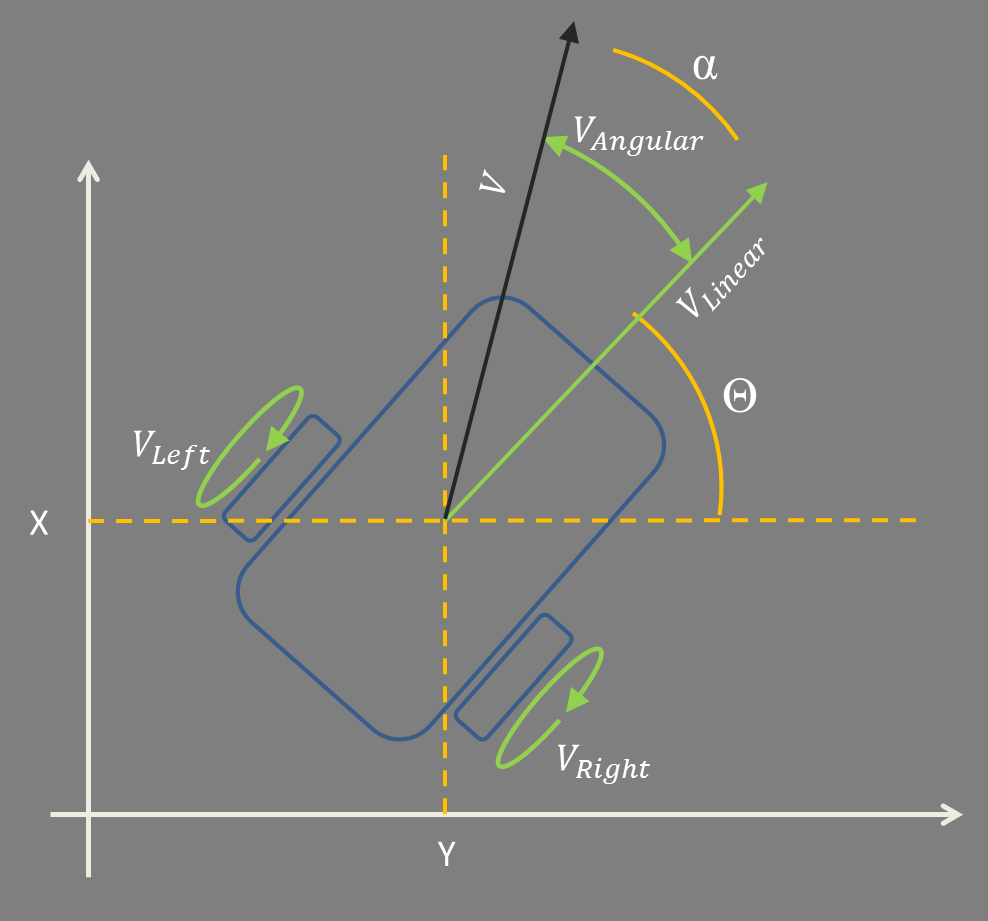
\includegraphics[width=0.25\textwidth] {KinModel.png}
\end{center}
\caption{Kinematic Model of Non-holonomic Differential Drive Robot}
\label{fig:KinModel}
\end{figure}
\begin{align}
V & =k_{att}.(Pos_{current}-Pos_{destination})\\
V_{linear} &= \begin{Vmatrix}v\end{Vmatrix} cos(\theta) ,
V_{angular} = {K\theta \over \pi}\\
V_{left}&=V_{Linear}-rsin(V_{Angular})\\
V_{right}&=V_{Linear}+rsin(V_{Angular})
\end{align}

Integrating all this we were able to implement a successful motion planning algorithm which distinguished our team from other teams.\linebreak

\subsubsection{Results}
A sample result of running this algorithm on the pitch is demonstrated in figure \ref{fig:seq}, Overall, this algorithm could deal with almost all scenarios successfully and when integrated with a high level decision making layer, we had a reliable game play scenario. 
The solution also can also deal effectively with obstacles using Extended Potential Field algorithm\cite{paper:OKhatib} but this feature was not used because obstacle avoidance was dealt with by higher levels of decision making. Therefore, the algorithm at this level is a conventional P controller.  

\begin{figure}[!bp]
\begin{center}
\subfigure[]{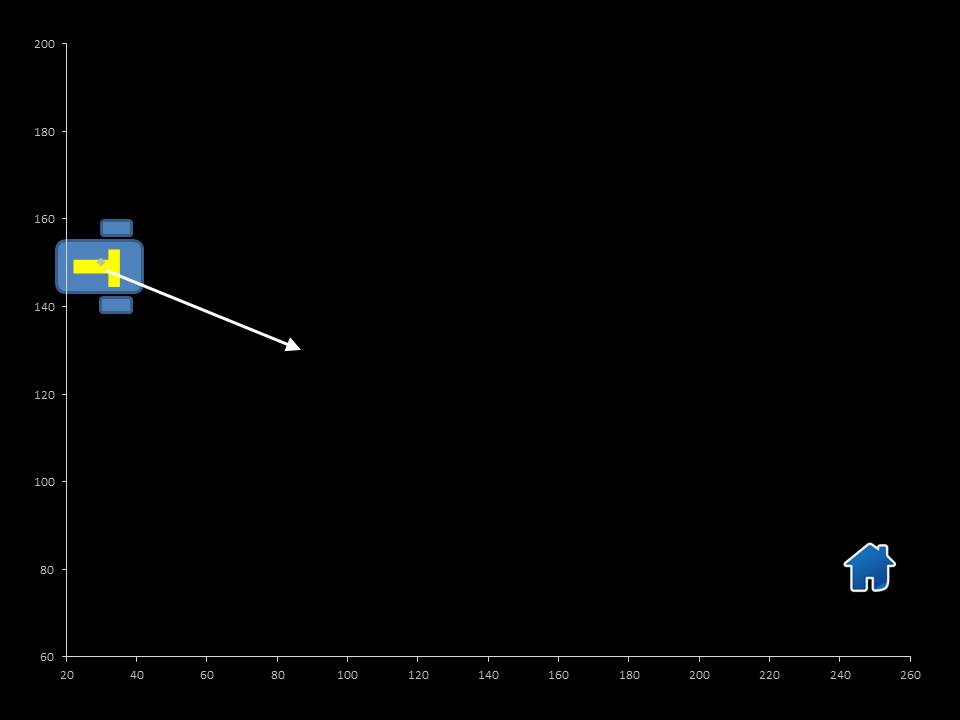
\includegraphics[width=0.15\textwidth] {step1.jpg}}
\subfigure[]{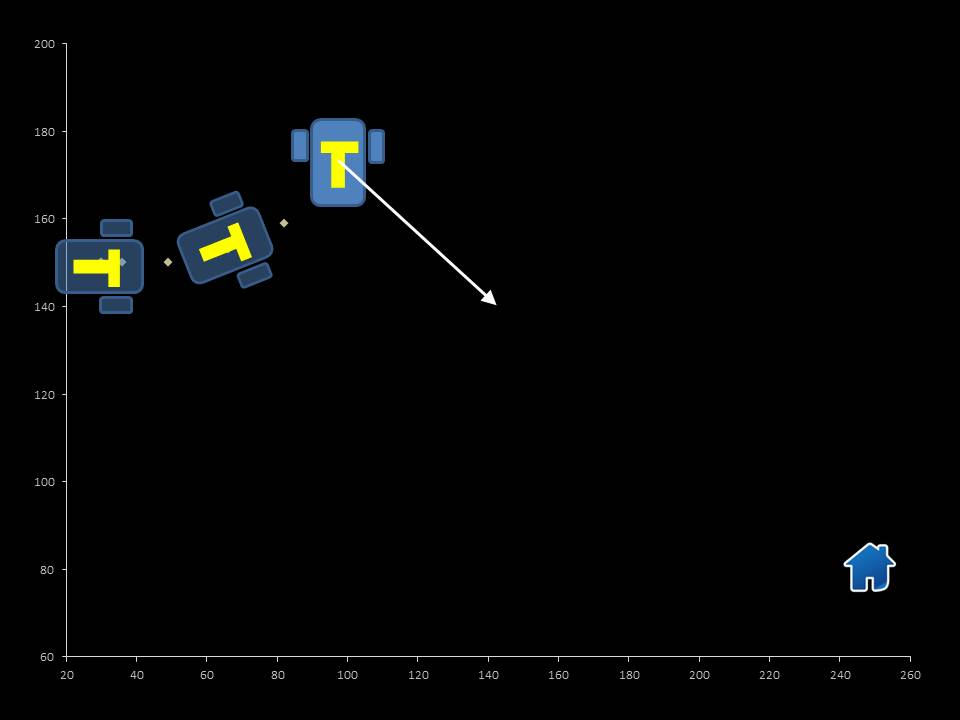
\includegraphics[width=0.15\textwidth] {step2.jpg}}
\subfigure[]{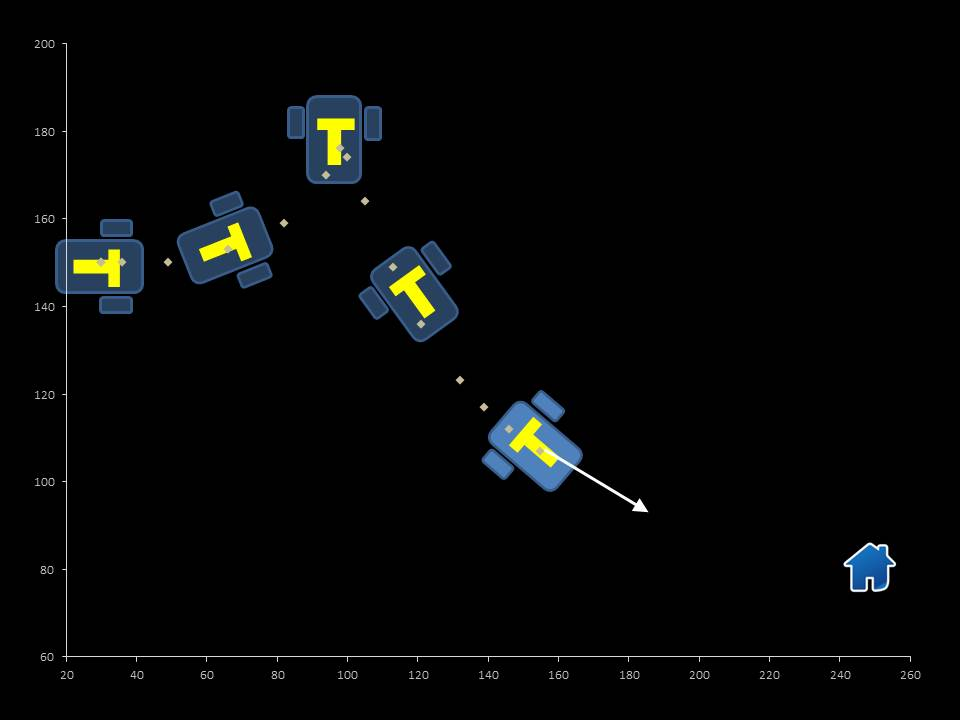
\includegraphics[width=0.15\textwidth] {step3.jpg}}
\subfigure[]{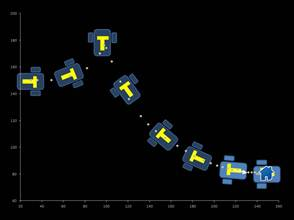
\includegraphics[width=0.15\textwidth] {Final.jpg}}
\caption{A sequence of robot movements from start position to destination.}
\label{fig:seq}
\end{center}
\end{figure}

\subsubsection{Lessons Learned}

\begin{itemize}
\item It is possible to implement reliable applications based on ideas developed in research labs. 
\item Failure of an algorithm at higher levels sometimes may be due to invalid inputs from lower layers.
\item Simulation at abstract level is very useful for making sure that an algorithm is developed according to specification but successful implementation based on such simulation environments does does not guarantee optimal performance in real environments.
\end{itemize}
\section{Simulator}

Soon after the first models of the robot were developed we began to think about the behaviour of the robot. It became apparent that the strategy team could benefit a lot from having a medium on which to make quick tests, instead of having to depend on the availability of the pitch. Consequently, a decision was made to build a simulator. Considering Java was the main language of the project, Java Swing was chosen as it is the primary Java GUI toolkit.\linebreak

The aim in designing the simulator was to imitate a pitch environment so that strategies could undergo preliminary debugging. Real pictures of the pitch, the ball and the robots, were taken and then used so that proportions didn’t have to be considered. As the goal of the simulation was to mimic the real robot and its use of  non-holonomic differential drive wheels, forward kinematics, which considered the speed of the wheels, were used to compute the robot’s future position and orientation.\linebreak
formulas for behzad to put
A problem that occurred using this model was that if the speed of the left and right wheels were equal, the denominator in the equation is zero. One approach is to use a different approximation formula for this special case. It was decided that this is unneeded complication. Therefore, in order to have perfectly straight movement if the wheel speeds were equal, a very small floating point number was subtracted from one of the wheel speeds.\linebreak

For collision detection, there was an initial attempt at using an external physics library. However, the team’s usage of the simulator was very specific, a custom made physics library was made purely for these targeted purposes. Objects requiring collision detection needed to implement a CollisionListener class and are then registered with a central CollisionDetector. The CollisionDetector stores the objects into an ArrayList and loops through them. Each object registered must have a shape and each corner of every shape is checked for inclusion in any other object shape. If this is the case, both objects are notified and sent a Collision packet describing the specifics of the collision. The different objects handle their own specific collisions: the ball bounces off the walls of the pitch, the robots collide with each other and the walls, and the kicker kicks the ball at the angle the robot is facing. \linebreak

In order to improve strategy debugging efficiency, a class was implemented so that the strategy code could access to the drawing capabilities of the simulator extremely easy. This class abstracts all of the work needed to draw on the simulator’s screen and provides a better alternative to the previously scattered console printing statements that clogged the code. We were now easily able to visualize the state of execution of any algorithm, any calculation, or any navigation points used in the strategy. \linebreak

Mouse and keyboard shortcuts provide further functionality. For instance, repositioning the objects on the pitch and enabling and disabling the robot in use. This first addition allowed us to immediately test the behavior of the strategy in any possible case. The second one allowed us to stop the robot from executing commands. As a result, we were able to easily examine the current state and parameters of the strategy because they would automatically drawn on the simulator. \linebreak

Although no direct quantitative measurement can be obtained, it was features like this that proved to be crucial in early testing, debugging and optimization. All the tools available in the simulator were heavily utilized by the strategy team. Coming up with ways of streamlining and facilitating testing, meant we were able to solve problems more quickly and more effectively.
\section{Perception}
The robot was able to perceive the environment it is situated in using the overhead camera. Using the images provided by the camera, we were able to calculate robot and opponent location and orientation, ball location on the pitch and the pitch itself.

\subsection{Initial approach}
Finding locations of different objects proved to be easy using simple methods like colour segmentation. The main challenge was in calculating robot orientation. Initially we used the dark spot and the T on the plate. This method was not very successful, since isolating the dark spot proved to be hard and inaccurate.
\subsection{Machine Learning}
Later a solution based on Machine-Learning methods was developed. We implemented solutions using SVM and Bayse algorithms available in the OpenCV library. A range of features such as hue moments, compactness and area were used for training a model for each object. We also used distance between two objects, by using this feature we were able to first find a principal object T and then using the distance feature find the correct dark spot close to this object.
\subsection{Central Image Moments}
Even though the Machine-Learning based solution produced reliable outputs but we realised that for a problem of this size, there should be simpler methods available. After studying the literature of computer vision, we implemented a method using second order of central image moments. This method is based on calculating main inertial axes, around which the object can be rotated with minimal or maximal inertia\ref{fig:SecondMethod}. For detailed description of this method reader is referred to\cite{Teague:80}. Using this method orientation of an object is computed as follows:
\begin{align}
\label{equ:centroid}
\mu'_{20} = \mu_{20} / \mu_{00} = M_{20}/M_{00} - \bar{x}^2 \\
\mu'_{02} = \mu_{02} / \mu_{00} = M_{02}/M_{00} - \bar{y}^2 \\
\mu'_{11} = \mu_{11} / \mu_{00} = M_{11}/M_{00} - \bar{x}\bar{y} \\
\Theta = \frac{1}{2} \arctan2 \left( {2\mu'_{11}},{\mu'_{20} - \mu'_{02}} \right) \label{orientationEq}
\end{align}
One can observe that equation 4 produces results from $-\pi/2$ - $\pi/2$. Our method cannot compute the heading of the calculated vector, to disambiguate this issue we used another method that was developed in earlier stages. It uses central moments of the object and the circle fitted around the object to calculate the orientation\ref{fig:CircleMethod}. This combined solution could produce reliable output. 
\begin{figure}[htp]
\begin{center}
\leavevmode
\subfigure[]{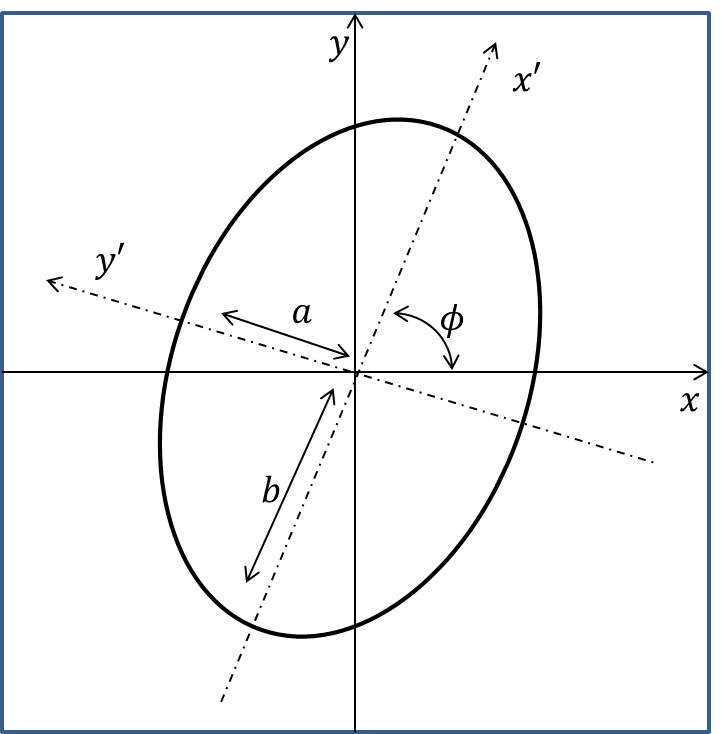
\includegraphics[width=0.15\textwidth] {secondOrderOrien.png}\label{fig:SecondMethod}}
\subfigure[]{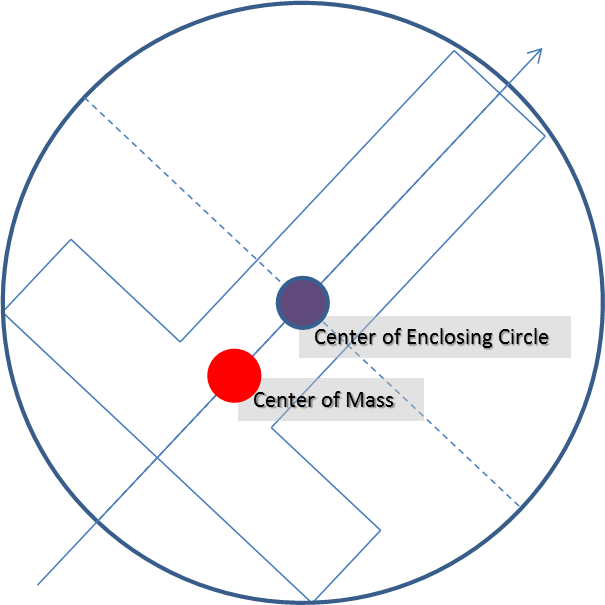
\includegraphics[width=0.15\textwidth]{CenOrien.png}\label{fig:CircleMethod}}
\end{center}
\caption{Calculating orientation using second order of central moments(a) and center of mass of object and surrounding circle(b)}
\end{figure} 
Even though our method calculating robot orientation was not very robust against noise at the specified areas, it was very accurate in 85 to 90\% of the cases. 
\subsection{Results}
Using second order of image moments for calculating orientation of objects was effective for this project. Implementing this method was one of the keys to our success in milestone 3(score 70) and first friendly match(becoming semi-finalist) and later in other
matches. Our initial implementations had a very poor performance of about 5fps, however by the end of the project and using simpler methods we reached frame rates of over 22fps. Our program however suffered from major drops in frame rates on some specific machines in the lab, we could not successfully resolve the issue since the problem was not easily reproducible. This issue was one the major reasons we could not perform very well in the final match. 
A few other achievements in this part of the project was to learn how to effectively use OpenCV library in C. We also learned about Bayes and SVM classifiers and compare their performance.
The developed library contains:
\begin{itemize}
\item Various methods of object isolation methods such as background subtraction and colour segmentation. Various methods of calculating orientation as described earlier.
\item Complete implementation of Machine Learning methods for object recognition.
\item Utility programs for tuning the colour segmentation thresholds.
\item Utility methods for changing functionality of program based on input parameters.
\end{itemize}
\begin{figure}[htp]
\begin{center}
\leavevmode
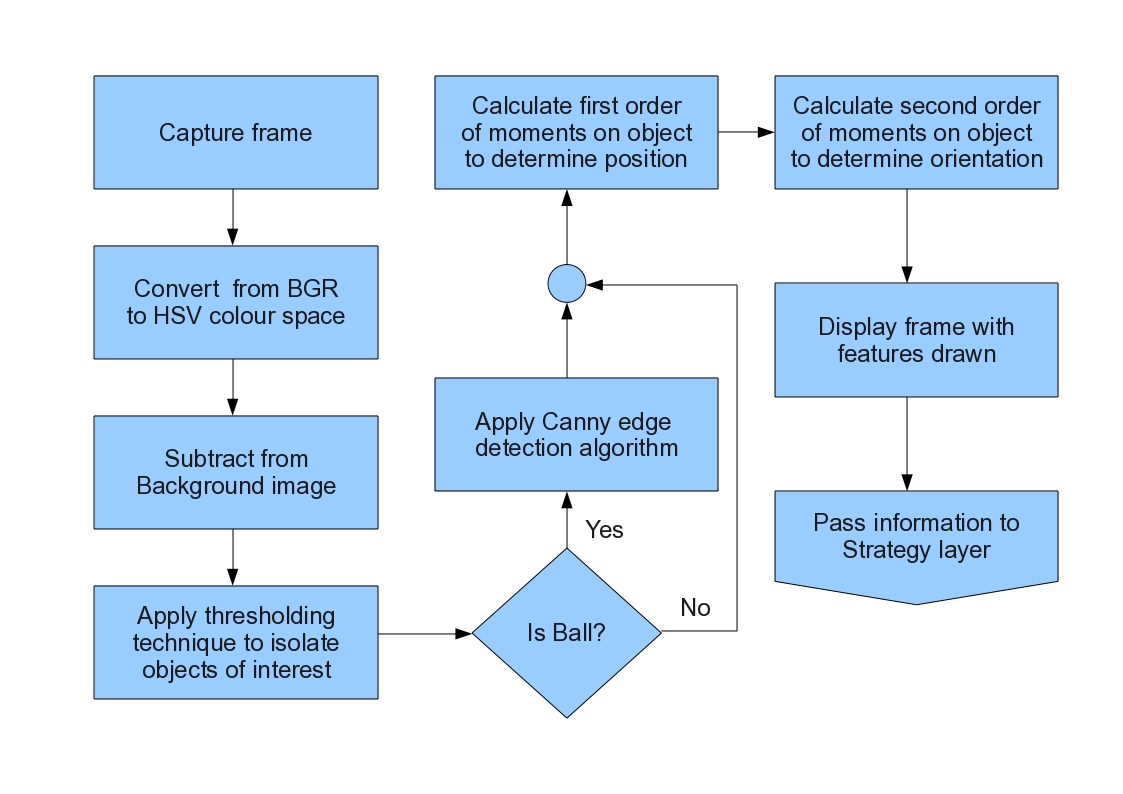
\includegraphics[width=0.4\textwidth] {vision_stack.jpg}
\end{center}
\caption{Final flow chart of vision program}
\label{fig:CircleMethod}
\end{figure}
\section{Low Level Motion}
In low level motion planning layer of the agent architecture we needed a robust algorithm capable of compensating possible noise incurred by output of vision stack.  The simple goal for this part is to make robot capable of following a path to reach a destination position determined by higher levels of path planning algorithm.
\subsection{Potential Field}
To achieve the goal stated above we started with implementing Potential Fields\cite{paper:PF} algorithm. This algorithm is a well-known method for robot path planning. It has several properties which makes it suitable for our application. The behaviour of the algorithm is completely reactive and therefore if it is fed with noisy input in one cycle it will be able to recover in next cycles, therefore performance of the algorithm degrades as amount of noise increases never failing completely.
\subsection{Challenges}
During implementation of this method, we had several challenges. We started testing this algorithm for milestone two but failed. The initial intuition for most members was that the failure was due to complexity of this algorithm while the failure was in fact due to unreliable input produced by vision stack. Later, new set of tests showed a very good performance once the vision stack become robust and reliable. Successful implementation of this algorithm was a key to our success in third and fourth friendly matches.
\subsection{Kinematic Model and Implementation}
In order to implement this algorithm successfully we needed to find a way to apply the calculated velocity vector from previous step on the robot. To do this, we used a kinematic model of a differential drive robot. In figure \ref{KinModel},the velocity vector is decomposed into linear and angular velocity and later they are fused to calculate velocity of left and right wheels.
\begin{figure}[htp]
\begin{center}
\leavevmode
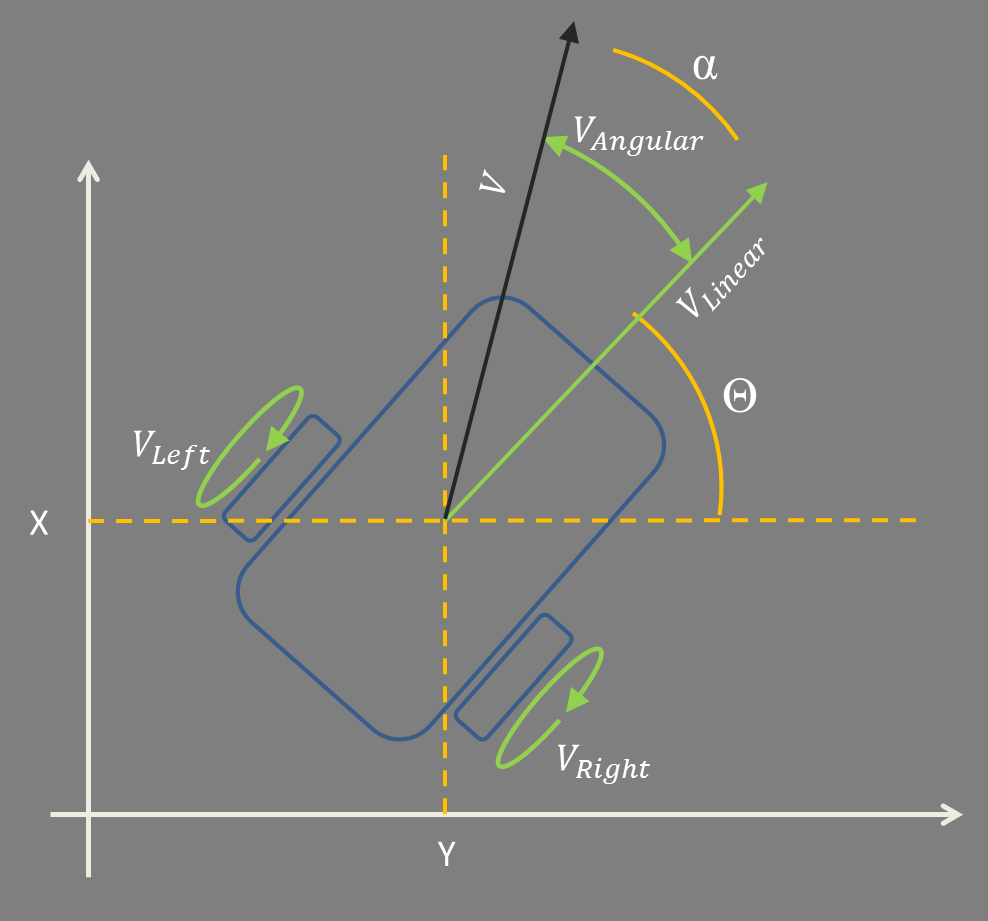
\includegraphics[width=0.25\textwidth] {KinModel.png}
\end{center}
\caption{Kinematic Model of Non-holonomic Differential Drive Robot}
\label{fig:KinModel}
\end{figure}
\begin{align}
V & =k_{att}.(Pos_{current}-Pos_{destination})\\
V_{linear} &= \begin{Vmatrix}v\end{Vmatrix} cos(\theta) ,
V_{angular} = {K\theta \over \pi}\\
V_{left}&=V_{Linear}-rsin(V_{Angular})\\
V_{right}&=V_{Linear}+rsin(V_{Angular})
\end{align}

Integrating all this we were able to implement a successful motion planning algorithm which distinguished our team from other teams.
\subsection{Results and Lessons Learned}
A sample result of running this algorithm on the pitch is demonstrated in figure \ref{fig:seq}, Overall, this algorithm could deal with almost all scenarios successfully and when integrated with a high level decision making layer, we had a reliable game play scenario. 
The solution also can also deal effectively with obstacles using Extended Potential Field algorithm\cite{paper:OKhatib} but this feature was not used because obstacle avoidance was dealt with by higher levels of decision making. Therefore, the algorithm at this level is a conventional P controller.  

\begin{figure}[htp]
\begin{center}
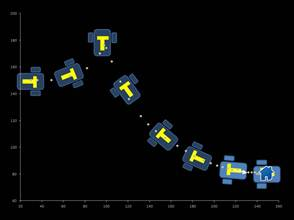
\includegraphics[width=0.25\textwidth] {Final.jpg}
\caption{Complete Robot movements from start position to destination position.}
\label{fig:seq}
\end{center}
\end{figure}
\subsection{Lessons Learned}

\begin{itemize}
\item It is possible to implement reliable applications based on ideas developed in research labs. 
\item Failure of an algorithm at higher levels sometimes may be due to invalid inputs from lower layers.
\item Simulation at abstract level is very useful for making sure that an algorithm is developed according to specification but successful implementation based on such simulation environments does does not guarantee optimal performance in real environments.
\end{itemize}
\bibliographystyle{IEEEtran}
\bibliography{bibliography}
% An example of a floating figure using the graphicx package.
% Note that \label must occur AFTER (or within) \caption.
% For figures, \caption should occur after the \includegraphics.
% Note that IEEEtran v1.7 and later has special internal code that
% is designed to preserve the operation of \label within \caption
% even when the captionsoff option is in effect. However, because
% of issues like this, it may be the safest practice to put all your
% \label just after \caption rather than within \caption{}.
%
% Reminder: the "draftcls" or "draftclsnofoot", not "draft", class
% option should be used if it is desired that the figures are to be
% displayed while in draft mode.
%
%\begin{figure}[!t]
%\centering
%\includegraphics[width=2.5in]{myfigure}
% where an .eps filename suffix will be assumed under latex, 
% and a .pdf suffix will be assumed for pdflatex; or what has been declared
% via \DeclareGraphicsExtensions.
%\caption{Simulation Results}
%\label{fig_sim}
%\end{figure}

% Note that IEEE typically puts floats only at the top, even when this
% results in a large percentage of a column being occupied by floats.


% An example of a double column floating figure using two subfigures.
% (The subfig.sty package must be loaded for this to work.)
% The subfigure \label commands are set within each subfloat command, the
% \label for the overall figure must come after \caption.
% \hfil must be used as a separator to get equal spacing.
% The subfigure.sty package works much the same way, except \subfigure is
% used instead of \subfloat.
%
%\begin{figure*}[!t]
%\centerline{\subfloat[Case I]\includegraphics[width=2.5in]{subfigcase1}%
%\label{fig_first_case}}
%\hfil
%\subfloat[Case II]{\includegraphics[width=2.5in]{subfigcase2}%
%\label{fig_second_case}}}
%\caption{Simulation results}
%\label{fig_sim}
%\end{figure*}
%
% Note that often IEEE papers with subfigures do not employ subfigure
% captions (using the optional argument to \subfloat), but instead will
% reference/describe all of them (a), (b), etc., within the main caption.


% An example of a floating table. Note that, for IEEE style tables, the 
% \caption command should come BEFORE the table. Table text will default to
% \footnotesize as IEEE normally uses this smaller font for tables.
% The \label must come after \caption as always.
%
%\begin{table}[!t]
%% increase table row spacing, adjust to taste
%\renewcommand{\arraystretch}{1.3}
% if using array.sty, it might be a good idea to tweak the value of
% \extrarowheight as needed to properly center the text within the cells
%\caption{An Example of a Table}
%\label{table_example}
%\centering
%% Some packages, such as MDW tools, offer better commands for making tables
%% than the plain LaTeX2e tabular which is used here.
%\begin{tabular}{|c||c|}
%\hline
%One & Two\\
%\hline
%Three & Four\\
%\hline
%\end{tabular}
%\end{table}


% Note that IEEE does not put floats in the very first column - or typically
% anywhere on the first page for that matter. Also, in-text middle ("here")
% positioning is not used. Most IEEE journals/conferences use top floats
% exclusively. Note that, LaTeX2e, unlike IEEE journals/conferences, places
% footnotes above bottom floats. This can be corrected via the \fnbelowfloat
% command of the stfloats package.

% conference papers do not normally have an appendix


% use section* for acknowledgement




% trigger a \newpage just before the given reference
% number - used to balance the columns on the last page
% adjust value as needed - may need to be readjusted if
% the document is modified later
%\IEEEtriggeratref{8}
% The "triggered" command can be changed if desired:
%\IEEEtriggercmd{\enlargethispage{-5in}}

% references section

% can use a bibliography generated by BibTeX as a .bbl file
% BibTeX documentation can be easily obtained at:
% http://www.ctan.org/tex-archive/biblio/bibtex/contrib/doc/
% The IEEEtran BibTeX style support page is at:
% http://www.michaelshell.org/tex/ieeetran/bibtex/
%\bibliographystyle{IEEEtran}
% argument is your BibTeX string definitions and bibliography database(s)
%\bibliography{IEEEabrv,../bib/paper}
%
% <OR> manually copy in the resultant .bbl file
% set second argument of \begin to the number of references
% (used to reserve space for the reference number labels box)
%\begin{thebibliography}{1}

%\bibliographystyle{IEEEtran}
%\bibliography{bibliography}

%\end{thebibliography}




% that's all folks
\end{document}


